The system's LTS visualization can be checked for determining the absence of deadlocks, and the system can be verified using $\mu$-calculus formulas to verify the plain text requirements stated previously. \texttt{mcf} files are used to verify the requirements translated to $\mu$-calculus formulas.

\section{Tools used for verification}

The MCRL2 version used for performing the modelling and verification of the system is 201808.0.\\

A makefile has been created and used to make performing the verification tests easier. It is included in the zip archive and the accompanying readme file explains how it is to be used.\\
\texttt{mcrl22lps} is used for generating the lps file, and the \texttt{lps2lts} command is used for generating the corresponding lts file.

\section{Verification process}
Once the lps is generated, we call lps2pbes on it for every MCF ($\mu$-calculus formula) file corresponding to each of the safety and liveness requirements.\\
Once we have the .pbes files, we call \texttt{pbes2bool} on each of them so as to get a boolean value representing whether the test condition holds or not. Ideally, in order to say that our requirements have been met, we would want each \texttt{pbes2bool} call to return a \textit{true} value.\\\\
As expected, in our system, running the requirements tests through the MCF files returns a \textit{true} in each case, thus proving that all the requirements are met.\\\\
We tried running a variant with no communications enabled between the components, and two of the liveness requirements fail by returning a false, as expected. However, one of the liveness requirements does not rely on communication between the components and hence it returned a true. But we can clearly see that all the liveness requirements were not met in that case.

\section{Deadlock absence verification}
The system's LTS is used to generate a 3D figure of the state-space using the \texttt{ltsview} command, and the figure can be used to verify the absence of deadlocks through a visual inspection (a "Mark deadlocks" option in the MCRL2 GUI shows deadlocks present in the system, if any, as red spheres).
Moreover, the $\mu$-calculus formula for showing that a system is deadlock-free is: $[true*] \langle true \rangle true$ - it should return a true if there are no deadlocks.
\\\\
In our case, the visualization rendered does not show any deadlocks, as can be seen below:
\begin{figure}[h]
\centering
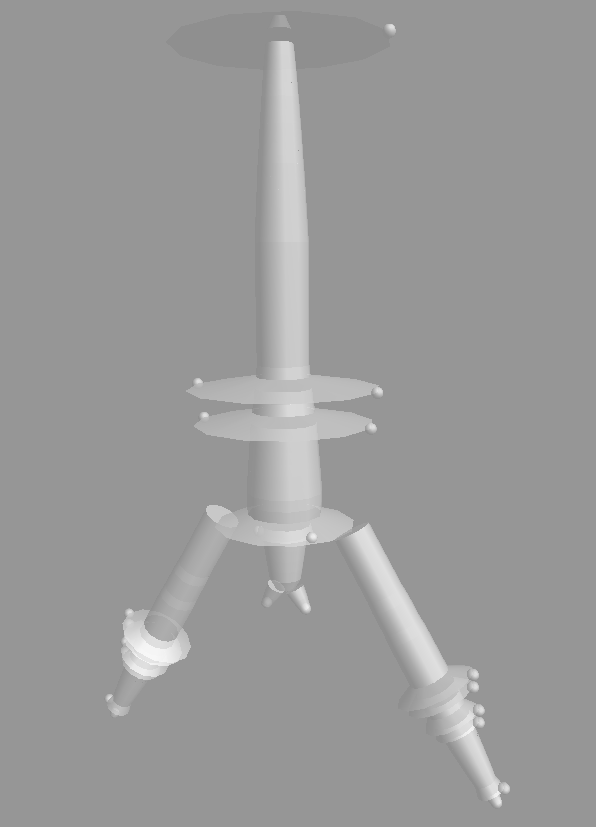
\includegraphics[width=70mm]{img/ltsview-nodeadlocks.PNG}
\caption{LTS view marking deadlocks\label{fig:ltsviewnodeadlocks}}
\end{figure}

The $\mu$-calculus formula returns true for our system, and hence we can say that our system is deadlock-free.

The LTS generated can be visualized in the form of a 3D shape using the \texttt{ltsview} command on the previously generated lts file.